\documentclass[12pt]{article}

\usepackage[portuguese,linesnumbered,ruled,vlined]{algorithm2e}
\usepackage{sbc-template}
\usepackage{graphicx,url,amsfonts}

\usepackage[brazil]{babel}
\usepackage[utf8]{inputenc}
\usepackage{hyperref}

\pagenumbering{arabic}

\sloppy

\title{Trabalho Prático de Programação Natural\\Cubo Mágico}

\author{Gabriel de Biasi\inst{1}}

\address{
Departamento de Ciência da Computação\\
Universidade Federal de Minas Gerais\\
Av. Antônio Carlos, 6627 -- Pampulha -- Belo Horizonte -- MG
\email{biasi@dcc.ufmg.br}
}

\begin{document}

\maketitle

\section{Descrição do Problema}
  O brinquedo ``Cubo Mágico'' ou \textit{Rubik's Cube} foi criado por Rubik em 1974 e distribuído comercialmente em 1980. Possui um conjunto de 26 cubos menores, 6 faces com três tipos de cubos distintos: São 4 centros, 12 meios e 8 quinas. Cada tipo cubo possui um número específico de cores, onde os centros possui uma cor, meios possuem duas cores e as quinas possuem três cores.

  É possível realizar movimentos em faces do cubo mágico sendo possível rotacionar os cubos desta face. Há 3 movimentos distintos que podem ser feitos em cada face, sendo eles: rotação horária, rotação anti-horária e dupla rotação. Logo, o cubo mágico tem um total de 18 movimentos possíveis. O objetivo do jogo é fazer com que todas as faces tenham a mesma cor. Na \autoref{fig:cube} temos na esquerda um cubo em um estado ``bagunçado'' e outro no estado concluído.


  \begin{figure}[!ht]
    \centering
    \caption{Cubo mágico bagunçado e um cubo mágico resolvido}
    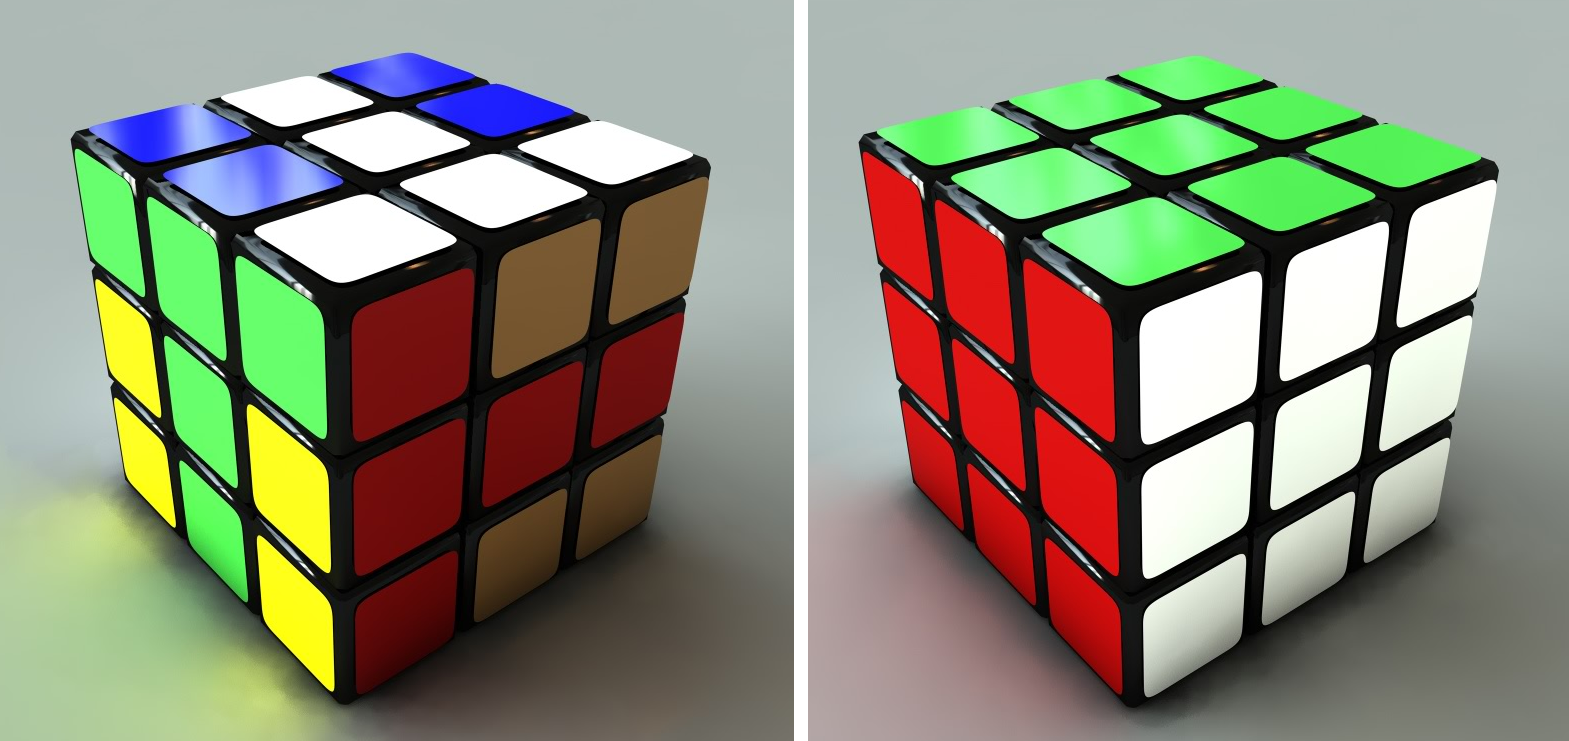
\includegraphics[scale=0.3]{images/cube.png}
    \label{fig:cube}
  \end{figure}

  Neste trabalho, é proposto um algoritmo evolutivo que tenha capacidade de resolver uma dada instância de cubo mágico colocando-o no estado resolvido e ao mesmo tempo buscando minimizar a quantidade de movimentos necessários.

\section{Metodologia}
  Para alcançar o objetivo do jogo, foi utilizado como base um método de resolução criado pelo professor \textit{Morwen Thistlethwaite}, onde o espaço de buscas de soluções é categorizado e então o cubo precisa ser levado de uma categoria para a próxima utilizando apenas os movimentos permitidos da categoria atual \cite{thistlethwaite}.

  \subsection{Categorias do Cubo}
    Thistlethwaite criou 5 categorias, que descreve o tão próximo um cubo mágico está da solução. As categorias diminuem drasticamente o espaço de busca de soluções, fazendo com que a busca pela solução simplifique com o avanço entre as categorias.

    \begin{description}
      \item [G0] Todos os estados do cubo mágico possíveis. Naturalmente, todos os cubos mágicos já estão presentes no conjunto G0. Sua ordem é de $|G0| = 4.33 \times 10^{19}$.
      \item [G1] Nesta categoria, os meios do cubo estão devidamente \textbf{orientados}, ou seja, não são necessários os movimentos simples $[L, R]$ para colocá-los em sua posição original. Sua ordem é de $|G1| = 2.11 \times 10^{19}$.
      \item [G2] Na categoria G2 os meios da camada do meio não podem ser movidos de suas faces e a face de cima e a face de baixo só possuem suas respectivas cores amarelo/branco. Sua ordem é de $|G2| = 1.95 \times 10^{10}$.
      \item [G3] Todas as faces opostas do cubo mágico agora possuem suas determinadas cores. As faces frente/atrás terão laranja ou vermelho, cima/baixo terão amarelo ou branco e esquerda/direita terão verde ou azul. Sua ordem é de $|G3| = 6.63 \times 10^{5}$.
      \item [G4] Estado do cubo resolvido, $|G4| = 1$.
    \end{description}






  Os movimentos de cada categoria que permitem levar para a próxima sem a quebra de propriedade são os seguintes:

  \begin{table}[ht]
      \centering
      \caption{Movimentos permitidos em cada categoria}
      \begin{tabular}{|c|c|}
        \hline
        \textbf{Categoria} & \textbf{Conjunto de Movimentos Permitidos}  \\ \hline
            G0             &  $(F, R, U, B, L, D)$           \\ \hline
            G1             &  $(F, R, U, B, L2, D2)$         \\ \hline
            G2             &  $(F, R, U2, B2, L2, D2)$       \\ \hline
            G3             &  $(F2, R2, U2, B2, L2, D2)$     \\ \hline
            G4             &  $\emptyset$                    \\ \hline
      \end{tabular}
  \end{table}

  \cite{thistlethwaiteES}.

\section{Descrição Geral da Implementação}
  Nesta seção, será discutido como as funções básicas de algoritmos evolucionários foram implementadas para o contexto do problema proposto.

  \subsection{Fluxo de Trabalho do Algoritmo}
    O algoritmo inicia com a definição de três constantes, $Alpha\ (\alpha)$, $Theta\ (\Theta)$ e $Lambda\ (\lambda)$. Estas constantes representam, respectivamente, a quantidade de gerações máxima do algoritmo, o tamanho da população e a quantidade de indivíduos resolvidos necessária para avançar uma categoria.

  \subsection{Definição de um Indivíduo}
    Neste algoritmo, um indivíduo é representado por uma lista de movimentos no cubo mágico, partindo do estado do cubo que foi passado quando o algoritmo iniciou. Exemplo:

      \begin{table}[ht]
      \centering
      \caption{Exemplos de Indivíduos}
      \begin{tabular}{|c|c|}
        \hline
        \textbf{ID} & \textbf{Conjunto de Movimentos}             \\ \hline
            $I1$             &  $[F, R2, Ui, B, L2,\dots, D, Fi]$ \\ \hline
            $I2$             &  $[Di, Ui, R2, D2, U, Li]$         \\ \hline
            $I3$             &  $[U2, R2, Ui, D, F2]$             \\ \hline
            $I4$             &  $[\emptyset]$                     \\ \hline
      \end{tabular}
      \end{table}

    É importante ressaltar que cada indivíduo deste algoritmo evolucionário possui \textbf{quatro} valores de $fitness$ diferentes, que é melhor explicado na \autoref{fit}.

 
  \subsection{Seleção}
    A seleção de indivíduos é feita por ranqueamento simples, onde todos os todos indivíduos da população atual são ordenados por $fitness$ e os $\lambda$ primeiros indivíduos
    são selecionados e considerados os candidatos para gerar a próxima geração.

    Após a seleção, todos $\lambda$ candidatos terão a probabilidade $\frac{1}{\lambda}$ de serem escolhidos e então serem duplicados. Este processo se repete até que a nova população alcance a quantidade de $\Theta$ indivíduos.


  \subsection{Mutação}
    Etc.


  \subsection{Função $clean$} \label{clean}
    Esta função é chamada toda vez que uma sequência de mutação é criada para um indivíduo. A fim de reduzir o número de movimentos necessários para resolver o cubo mágico, movimentos em sequência que não geram efeitos no cubo são removidos e movimentos que podem ser simplificados são alterados, sem perda de contexto final do cubo.
    
    A seguir, temos três exemplos de simplificação que podem ser feitos em uma sequência de movimentos. Na \autoref{tab_clean} apenas o movimento $F$ é apresentado, entretanto estas regras podem ser utilizadas para quaisquer movimentos do cubo mágico e em qualquer ordem.

    \begin{table}[ht]
      \centering
      \caption{Exemplos de Reduções de Movimentos} \label{tab_clean}
      \begin{tabular}{|c|c|c|}
        \hline
        \textbf{Inicial} & \textbf{Motivo}              & \textbf{Final}    \\ \hline
            $[F, Fi]$    &  Não produz efeito           &  $[\emptyset]$    \\ \hline
            $[F, F]$     &  Torna-se um giro duplo      &  $[F2]$           \\ \hline
            $[F, F2]$    &  Torna-se um giro invertido  &  $[Fi]$           \\ \hline
      \end{tabular}
    \end{table}

  \subsection{Função $fitness$} \label{fit}
  

\section{Execução dos Experimentos}
  lala

\section{Conclusão}
  Neste trabalho.

\bibliographystyle{sbc}
\bibliography{ref}

\end{document}
